% Options for packages loaded elsewhere
\PassOptionsToPackage{unicode}{hyperref}
\PassOptionsToPackage{hyphens}{url}
%
\documentclass[
]{article}
\usepackage{lmodern}
\usepackage{amssymb,amsmath}
\usepackage{ifxetex,ifluatex}
\ifnum 0\ifxetex 1\fi\ifluatex 1\fi=0 % if pdftex
  \usepackage[T1]{fontenc}
  \usepackage[utf8]{inputenc}
  \usepackage{textcomp} % provide euro and other symbols
\else % if luatex or xetex
  \usepackage{unicode-math}
  \defaultfontfeatures{Scale=MatchLowercase}
  \defaultfontfeatures[\rmfamily]{Ligatures=TeX,Scale=1}
\fi
% Use upquote if available, for straight quotes in verbatim environments
\IfFileExists{upquote.sty}{\usepackage{upquote}}{}
\IfFileExists{microtype.sty}{% use microtype if available
  \usepackage[]{microtype}
  \UseMicrotypeSet[protrusion]{basicmath} % disable protrusion for tt fonts
}{}
\makeatletter
\@ifundefined{KOMAClassName}{% if non-KOMA class
  \IfFileExists{parskip.sty}{%
    \usepackage{parskip}
  }{% else
    \setlength{\parindent}{0pt}
    \setlength{\parskip}{6pt plus 2pt minus 1pt}}
}{% if KOMA class
  \KOMAoptions{parskip=half}}
\makeatother
\usepackage{xcolor}
\IfFileExists{xurl.sty}{\usepackage{xurl}}{} % add URL line breaks if available
\IfFileExists{bookmark.sty}{\usepackage{bookmark}}{\usepackage{hyperref}}
\hypersetup{
  pdftitle={Mise en forme et ingénierie des données},
  pdfauthor={Daniel Pont},
  hidelinks,
  pdfcreator={LaTeX via pandoc}}
\urlstyle{same} % disable monospaced font for URLs
\usepackage[margin=1in]{geometry}
\usepackage{color}
\usepackage{fancyvrb}
\newcommand{\VerbBar}{|}
\newcommand{\VERB}{\Verb[commandchars=\\\{\}]}
\DefineVerbatimEnvironment{Highlighting}{Verbatim}{commandchars=\\\{\}}
% Add ',fontsize=\small' for more characters per line
\usepackage{framed}
\definecolor{shadecolor}{RGB}{248,248,248}
\newenvironment{Shaded}{\begin{snugshade}}{\end{snugshade}}
\newcommand{\AlertTok}[1]{\textcolor[rgb]{0.94,0.16,0.16}{#1}}
\newcommand{\AnnotationTok}[1]{\textcolor[rgb]{0.56,0.35,0.01}{\textbf{\textit{#1}}}}
\newcommand{\AttributeTok}[1]{\textcolor[rgb]{0.77,0.63,0.00}{#1}}
\newcommand{\BaseNTok}[1]{\textcolor[rgb]{0.00,0.00,0.81}{#1}}
\newcommand{\BuiltInTok}[1]{#1}
\newcommand{\CharTok}[1]{\textcolor[rgb]{0.31,0.60,0.02}{#1}}
\newcommand{\CommentTok}[1]{\textcolor[rgb]{0.56,0.35,0.01}{\textit{#1}}}
\newcommand{\CommentVarTok}[1]{\textcolor[rgb]{0.56,0.35,0.01}{\textbf{\textit{#1}}}}
\newcommand{\ConstantTok}[1]{\textcolor[rgb]{0.00,0.00,0.00}{#1}}
\newcommand{\ControlFlowTok}[1]{\textcolor[rgb]{0.13,0.29,0.53}{\textbf{#1}}}
\newcommand{\DataTypeTok}[1]{\textcolor[rgb]{0.13,0.29,0.53}{#1}}
\newcommand{\DecValTok}[1]{\textcolor[rgb]{0.00,0.00,0.81}{#1}}
\newcommand{\DocumentationTok}[1]{\textcolor[rgb]{0.56,0.35,0.01}{\textbf{\textit{#1}}}}
\newcommand{\ErrorTok}[1]{\textcolor[rgb]{0.64,0.00,0.00}{\textbf{#1}}}
\newcommand{\ExtensionTok}[1]{#1}
\newcommand{\FloatTok}[1]{\textcolor[rgb]{0.00,0.00,0.81}{#1}}
\newcommand{\FunctionTok}[1]{\textcolor[rgb]{0.00,0.00,0.00}{#1}}
\newcommand{\ImportTok}[1]{#1}
\newcommand{\InformationTok}[1]{\textcolor[rgb]{0.56,0.35,0.01}{\textbf{\textit{#1}}}}
\newcommand{\KeywordTok}[1]{\textcolor[rgb]{0.13,0.29,0.53}{\textbf{#1}}}
\newcommand{\NormalTok}[1]{#1}
\newcommand{\OperatorTok}[1]{\textcolor[rgb]{0.81,0.36,0.00}{\textbf{#1}}}
\newcommand{\OtherTok}[1]{\textcolor[rgb]{0.56,0.35,0.01}{#1}}
\newcommand{\PreprocessorTok}[1]{\textcolor[rgb]{0.56,0.35,0.01}{\textit{#1}}}
\newcommand{\RegionMarkerTok}[1]{#1}
\newcommand{\SpecialCharTok}[1]{\textcolor[rgb]{0.00,0.00,0.00}{#1}}
\newcommand{\SpecialStringTok}[1]{\textcolor[rgb]{0.31,0.60,0.02}{#1}}
\newcommand{\StringTok}[1]{\textcolor[rgb]{0.31,0.60,0.02}{#1}}
\newcommand{\VariableTok}[1]{\textcolor[rgb]{0.00,0.00,0.00}{#1}}
\newcommand{\VerbatimStringTok}[1]{\textcolor[rgb]{0.31,0.60,0.02}{#1}}
\newcommand{\WarningTok}[1]{\textcolor[rgb]{0.56,0.35,0.01}{\textbf{\textit{#1}}}}
\usepackage{graphicx,grffile}
\makeatletter
\def\maxwidth{\ifdim\Gin@nat@width>\linewidth\linewidth\else\Gin@nat@width\fi}
\def\maxheight{\ifdim\Gin@nat@height>\textheight\textheight\else\Gin@nat@height\fi}
\makeatother
% Scale images if necessary, so that they will not overflow the page
% margins by default, and it is still possible to overwrite the defaults
% using explicit options in \includegraphics[width, height, ...]{}
\setkeys{Gin}{width=\maxwidth,height=\maxheight,keepaspectratio}
% Set default figure placement to htbp
\makeatletter
\def\fps@figure{htbp}
\makeatother
\setlength{\emergencystretch}{3em} % prevent overfull lines
\providecommand{\tightlist}{%
  \setlength{\itemsep}{0pt}\setlength{\parskip}{0pt}}
\setcounter{secnumdepth}{-\maxdimen} % remove section numbering

\title{Mise en forme et ingénierie des données}
\author{Daniel Pont}
\date{08/06/2020}

\begin{document}
\maketitle

{
\setcounter{tocdepth}{2}
\tableofcontents
}
\hypertarget{mise-en-forme-et-inguxe9nierie-des-donnuxe9es}{%
\section{Mise en forme et ingénierie des
données}\label{mise-en-forme-et-inguxe9nierie-des-donnuxe9es}}

\hypertarget{suxe9lection-des-donnuxe9es}{%
\subsection{1. Sélection des
données}\label{suxe9lection-des-donnuxe9es}}

\hypertarget{sous-ensemble-des-lignes-et-des-colonnes}{%
\subsubsection{1.1 Sous-ensemble des lignes et des
colonnes}\label{sous-ensemble-des-lignes-et-des-colonnes}}

Dans ce paragraphe, on souhaite étudier

\begin{Shaded}
\begin{Highlighting}[]
\KeywordTok{library}\NormalTok{(ggplot2)}
\KeywordTok{summary}\NormalTok{(iris)}
\end{Highlighting}
\end{Shaded}

\begin{verbatim}
##   Sepal.Length    Sepal.Width     Petal.Length    Petal.Width   
##  Min.   :4.300   Min.   :2.000   Min.   :1.000   Min.   :0.100  
##  1st Qu.:5.100   1st Qu.:2.800   1st Qu.:1.600   1st Qu.:0.300  
##  Median :5.800   Median :3.000   Median :4.350   Median :1.300  
##  Mean   :5.843   Mean   :3.057   Mean   :3.758   Mean   :1.199  
##  3rd Qu.:6.400   3rd Qu.:3.300   3rd Qu.:5.100   3rd Qu.:1.800  
##  Max.   :7.900   Max.   :4.400   Max.   :6.900   Max.   :2.500  
##        Species  
##  setosa    :50  
##  versicolor:50  
##  virginica :50  
##                 
##                 
## 
\end{verbatim}

\begin{Shaded}
\begin{Highlighting}[]
\KeywordTok{head}\NormalTok{(iris)}
\end{Highlighting}
\end{Shaded}

\begin{verbatim}
##   Sepal.Length Sepal.Width Petal.Length Petal.Width Species
## 1          5.1         3.5          1.4         0.2  setosa
## 2          4.9         3.0          1.4         0.2  setosa
## 3          4.7         3.2          1.3         0.2  setosa
## 4          4.6         3.1          1.5         0.2  setosa
## 5          5.0         3.6          1.4         0.2  setosa
## 6          5.4         3.9          1.7         0.4  setosa
\end{verbatim}

\begin{Shaded}
\begin{Highlighting}[]
\KeywordTok{ggplot}\NormalTok{(iris, }\KeywordTok{aes}\NormalTok{(}\DataTypeTok{x=}\NormalTok{Petal.Length,}\DataTypeTok{y=}\NormalTok{Petal.Width,}
                 \DataTypeTok{shape=}\NormalTok{ Species, }\DataTypeTok{color =}\NormalTok{ Species)) }\OperatorTok{+}
\StringTok{    }\KeywordTok{geom_point}\NormalTok{(}\DataTypeTok{size=}\DecValTok{2}\NormalTok{) }\OperatorTok{+}
\StringTok{    }\KeywordTok{ggtitle}\NormalTok{(}\StringTok{"Petal dimensions by iris species: all measurements"}\NormalTok{)}
\end{Highlighting}
\end{Shaded}

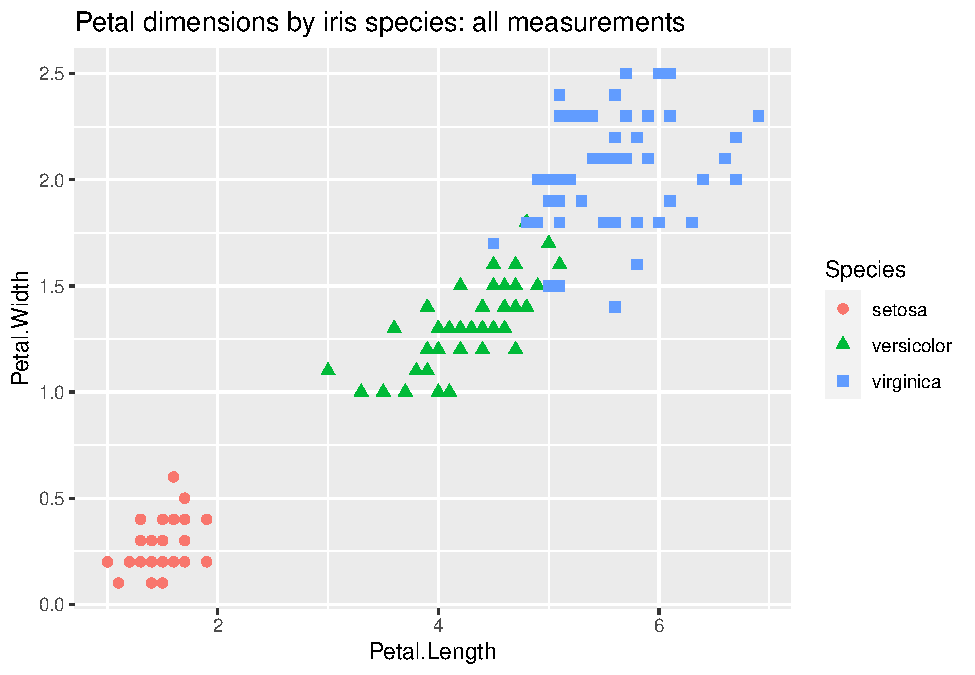
\includegraphics{5_Data_engineering_and_shaping_files/figure-latex/1.1-1.pdf}

\hypertarget{avec-les-muxe9thodes-de-base-en-r}{%
\paragraph{1.1.1 Avec les méthodes de base en
R}\label{avec-les-muxe9thodes-de-base-en-r}}

\begin{Shaded}
\begin{Highlighting}[]
\NormalTok{columns_we_want <-}\StringTok{ }\KeywordTok{c}\NormalTok{(}\StringTok{"Petal.Length"}\NormalTok{, }\StringTok{"Petal.Width"}\NormalTok{, }\StringTok{"Species"}\NormalTok{)}
\NormalTok{rows_we_want <-}\StringTok{ }\NormalTok{iris}\OperatorTok{$}\NormalTok{Petal.Length }\OperatorTok{>}\StringTok{ }\DecValTok{2}

\CommentTok{#AVANT}
\KeywordTok{head}\NormalTok{(iris)}
\end{Highlighting}
\end{Shaded}

\begin{verbatim}
##   Sepal.Length Sepal.Width Petal.Length Petal.Width Species
## 1          5.1         3.5          1.4         0.2  setosa
## 2          4.9         3.0          1.4         0.2  setosa
## 3          4.7         3.2          1.3         0.2  setosa
## 4          4.6         3.1          1.5         0.2  setosa
## 5          5.0         3.6          1.4         0.2  setosa
## 6          5.4         3.9          1.7         0.4  setosa
\end{verbatim}

\begin{Shaded}
\begin{Highlighting}[]
\CommentTok{#APRES}
\CommentTok{#(drop=false permet d'obtenir un data.frame et non un vector si on ne sélectionne qu'une seule colonne)}
\NormalTok{iris_base <-}\StringTok{ }\NormalTok{iris[rows_we_want,columns_we_want,drop=}\OtherTok{FALSE}\NormalTok{]}
\KeywordTok{head}\NormalTok{(iris_base)}
\end{Highlighting}
\end{Shaded}

\begin{verbatim}
##    Petal.Length Petal.Width    Species
## 51          4.7         1.4 versicolor
## 52          4.5         1.5 versicolor
## 53          4.9         1.5 versicolor
## 54          4.0         1.3 versicolor
## 55          4.6         1.5 versicolor
## 56          4.5         1.3 versicolor
\end{verbatim}

\hypertarget{avec-une-data.table}{%
\paragraph{1.1.2 Avec une data.table}\label{avec-une-data.table}}

Quelques points clés sur les data.tables :

\begin{itemize}
\tightlist
\item
  ce sont des méthodes d'indexation puissantes (ex. : ``..'' ci-dessous)
\item
  elles constitient la solution R la plus efficace en terme de rapidité
  et de de mémoire pour une large plage d'échelles
\item
  FAQ :
  \url{https://cran.r-project.org/web/packages/data.table/vignettes/datatable-faq.html}
\item
  Cheat sheet :
  \url{https://www.datacamp.com/community/tutorials/data-table-cheat-sheet}
\end{itemize}

\begin{Shaded}
\begin{Highlighting}[]
\KeywordTok{library}\NormalTok{(data.table)}
\NormalTok{iris_data.table <-}\StringTok{ }\KeywordTok{as.data.table}\NormalTok{(iris)}
\NormalTok{columns_we_want <-}\StringTok{ }\KeywordTok{c}\NormalTok{(}\StringTok{"Petal.Length"}\NormalTok{, }\StringTok{"Petal.Width"}\NormalTok{, }\StringTok{"Species"}\NormalTok{)}
\NormalTok{rows_we_want <-}\StringTok{ }\NormalTok{iris}\OperatorTok{$}\NormalTok{Petal.Length }\OperatorTok{>}\StringTok{ }\DecValTok{2}
\CommentTok{# .. indique que columns_we_want n'est pas un nom de colonne mais une varaible contenant les colonnes}
\NormalTok{iris_data.table <-}\StringTok{ }\NormalTok{iris_data.table[rows_we_want,..columns_we_want]}
\KeywordTok{head}\NormalTok{(iris_data.table)}
\end{Highlighting}
\end{Shaded}

\begin{verbatim}
##    Petal.Length Petal.Width    Species
## 1:          4.7         1.4 versicolor
## 2:          4.5         1.5 versicolor
## 3:          4.9         1.5 versicolor
## 4:          4.0         1.3 versicolor
## 5:          4.6         1.5 versicolor
## 6:          4.5         1.3 versicolor
\end{verbatim}

Pour mieux comprendre la notation ``..'', voici un exemple :

\begin{Shaded}
\begin{Highlighting}[]
\KeywordTok{library}\NormalTok{(data.table)}
\NormalTok{df <-}\StringTok{ }\KeywordTok{data.frame}\NormalTok{(}\DataTypeTok{x=}\DecValTok{1}\OperatorTok{:}\DecValTok{2}\NormalTok{,}\DataTypeTok{y=}\DecValTok{3}\OperatorTok{:}\DecValTok{4}\NormalTok{)}
\CommentTok{# ERREUR (x non défini) :}
\CommentTok{#df[,x]}

\CommentTok{#Fonctionnement avec une data.table :}
\NormalTok{dt <-}\StringTok{ }\KeywordTok{data.table}\NormalTok{(df)}
\NormalTok{x <-}\StringTok{ "y"}

\CommentTok{# sélectionne la colonne "x"}
\NormalTok{dt[,x]}
\end{Highlighting}
\end{Shaded}

\begin{verbatim}
## [1] 1 2
\end{verbatim}

\begin{Shaded}
\begin{Highlighting}[]
\CommentTok{# sélectionne la colonne "y"}
\NormalTok{dt[,..x]}
\end{Highlighting}
\end{Shaded}

\begin{verbatim}
##    y
## 1: 3
## 2: 4
\end{verbatim}

NB : Avec les packages qui ne les supportent pas, les data.tables se
comportent comme des data.frames.

\hypertarget{avec-dplyr}{%
\paragraph{1.1.3 Avec dplyr}\label{avec-dplyr}}

Pour sélectionner :

\begin{itemize}
\tightlist
\item
  des \emph{colonnes}, on utilise \emph{dplyr::select}
\item
  des \emph{lignes}, on utilise \emph{dplyr::filter}
\end{itemize}

\begin{Shaded}
\begin{Highlighting}[]
\KeywordTok{library}\NormalTok{(dplyr)}

\NormalTok{iris_dplyr <-}\StringTok{ }\NormalTok{iris }\OperatorTok\StringTok{ }
\StringTok{                }\KeywordTok{select}\NormalTok{( Petal.Length, Petal.Width, Species)  }\OperatorTok
\StringTok{                }\KeywordTok{filter}\NormalTok{( iris}\OperatorTok{$}\NormalTok{Petal.Length }\OperatorTok{>}\StringTok{ }\DecValTok{2}\NormalTok{)}
\CommentTok{# NB : on peut aussi utiliser  select( c("Petal.Length", "Petal.Width", "Species"))}

\KeywordTok{head}\NormalTok{(iris_dplyr)}
\end{Highlighting}
\end{Shaded}

\begin{verbatim}
##   Petal.Length Petal.Width    Species
## 1          4.7         1.4 versicolor
## 2          4.5         1.5 versicolor
## 3          4.9         1.5 versicolor
## 4          4.0         1.3 versicolor
## 5          4.6         1.5 versicolor
## 6          4.5         1.3 versicolor
\end{verbatim}

\hypertarget{suppression-des-enregistrements-avec-des-donnuxe9es-manquantes}{%
\subsubsection{1.2 Suppression des enregistrements avec des données
manquantes}\label{suppression-des-enregistrements-avec-des-donnuxe9es-manquantes}}

\begin{Shaded}
\begin{Highlighting}[]
\KeywordTok{library}\NormalTok{(ggplot2)}
\KeywordTok{data}\NormalTok{(msleep)}
\KeywordTok{str}\NormalTok{(msleep)}
\end{Highlighting}
\end{Shaded}

\begin{verbatim}
## tibble [83 x 11] (S3: tbl_df/tbl/data.frame)
##  $ name        : chr [1:83] "Cheetah" "Owl monkey" "Mountain beaver" "Greater short-tailed shrew" ...
##  $ genus       : chr [1:83] "Acinonyx" "Aotus" "Aplodontia" "Blarina" ...
##  $ vore        : chr [1:83] "carni" "omni" "herbi" "omni" ...
##  $ order       : chr [1:83] "Carnivora" "Primates" "Rodentia" "Soricomorpha" ...
##  $ conservation: chr [1:83] "lc" NA "nt" "lc" ...
##  $ sleep_total : num [1:83] 12.1 17 14.4 14.9 4 14.4 8.7 7 10.1 3 ...
##  $ sleep_rem   : num [1:83] NA 1.8 2.4 2.3 0.7 2.2 1.4 NA 2.9 NA ...
##  $ sleep_cycle : num [1:83] NA NA NA 0.133 0.667 ...
##  $ awake       : num [1:83] 11.9 7 9.6 9.1 20 9.6 15.3 17 13.9 21 ...
##  $ brainwt     : num [1:83] NA 0.0155 NA 0.00029 0.423 NA NA NA 0.07 0.0982 ...
##  $ bodywt      : num [1:83] 50 0.48 1.35 0.019 600 ...
\end{verbatim}

\begin{Shaded}
\begin{Highlighting}[]
\KeywordTok{summary}\NormalTok{(msleep)}
\end{Highlighting}
\end{Shaded}

\begin{verbatim}
##      name              genus               vore              order          
##  Length:83          Length:83          Length:83          Length:83         
##  Class :character   Class :character   Class :character   Class :character  
##  Mode  :character   Mode  :character   Mode  :character   Mode  :character  
##                                                                             
##                                                                             
##                                                                             
##                                                                             
##  conservation        sleep_total      sleep_rem      sleep_cycle    
##  Length:83          Min.   : 1.90   Min.   :0.100   Min.   :0.1167  
##  Class :character   1st Qu.: 7.85   1st Qu.:0.900   1st Qu.:0.1833  
##  Mode  :character   Median :10.10   Median :1.500   Median :0.3333  
##                     Mean   :10.43   Mean   :1.875   Mean   :0.4396  
##                     3rd Qu.:13.75   3rd Qu.:2.400   3rd Qu.:0.5792  
##                     Max.   :19.90   Max.   :6.600   Max.   :1.5000  
##                                     NA's   :22      NA's   :51      
##      awake          brainwt            bodywt        
##  Min.   : 4.10   Min.   :0.00014   Min.   :   0.005  
##  1st Qu.:10.25   1st Qu.:0.00290   1st Qu.:   0.174  
##  Median :13.90   Median :0.01240   Median :   1.670  
##  Mean   :13.57   Mean   :0.28158   Mean   : 166.136  
##  3rd Qu.:16.15   3rd Qu.:0.12550   3rd Qu.:  41.750  
##  Max.   :22.10   Max.   :5.71200   Max.   :6654.000  
##                  NA's   :27
\end{verbatim}

\hypertarget{avec-les-muxe9thodes-de-base-en-r-1}{%
\paragraph{1.2.1 Avec les méthodes de base en
R}\label{avec-les-muxe9thodes-de-base-en-r-1}}

\end{document}
